\section{How the trap is entered: a first-principles throughput curve}\label{sec:entry}

\begin{figure*}[t]\centering
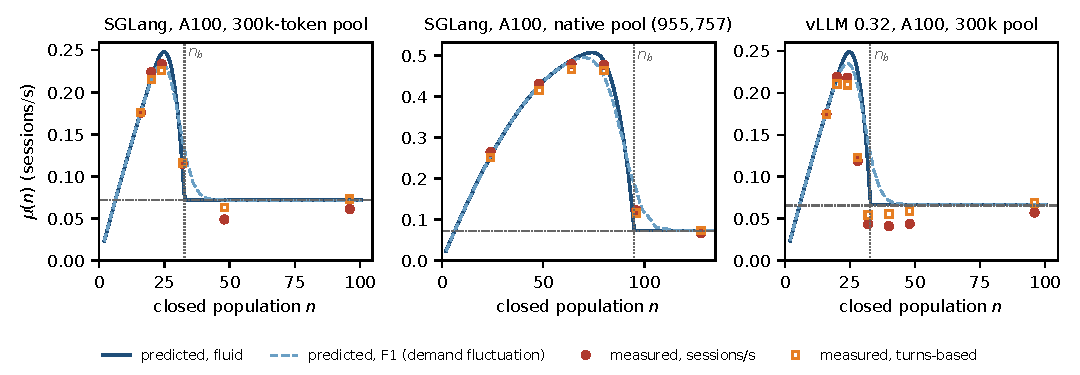
\includegraphics[width=\textwidth]{figs/fig8_theory_curves.pdf}
\caption{Predicted thrashing curves $\mu(n)$ against the engine. Lines: the first-principles model (solid, fluid; dashed, with
the demand-fluctuation layer F1), from the pool, the workload and a cost model fitted to server-log timing only; vLLM and the
H200 also get one speed factor fitted to their all-miss token rate. Points: measured $\mu(n)$, sessions/s (filled) and
turns-based (open). Dotted: the predicted all-miss onset $n_b$ (Proposition~\ref{prop:nb}); dash-dotted: the measured $\lref$. No
measured $\mu(n)$ point enters any prediction. The first three panels are in sample (the agents that derived the model knew
every point). The H200 panel is out of sample: predicted under tag \texttt{r13-theory-pred} before those agents read it; the runs at
$n=36$, 44 and 52 (ringed) are blind in time, those at $n\le32$ (shaded) had been seen by the first author, the others are blind
by access only (Appendix~\ref{app:frozen}).}\label{fig:fpmu}
\end{figure*}

Model~F describes the trap once it exists. Whether a load can be trapped at all is set by the closed-population throughput
curve $\mu(n)$, the session completion rate with $n$ sessions present: Denning's thrashing
curve~\citep{denning1968thrashing}. It rises with batching, peaks at $\mu^*$, and collapses to the all-miss level once
admitting waiting turns evicts the idle KV of sessions in tool calls. With open arrivals the classical quasi-static
approximation $\dot n=\lambda-\mu(n)$~\citep{courtois1975decomposability,kleinrock1975aloha} makes the good state metastable at
every load in the window $\mathcal W=(\lmiss,\min(\mu^*,\ledge))$, where $\ledge$ is the measured from-empty edge
(\S\ref{sec:fluid}); Lu et al.\ write the same population balance with an empirical hit curve~\citep{lu2026cachetrap}. We use it
for the window and the cap condition only, never for the trap.

\paragraph{The curve from first principles.} We predict $\mu(n)$ from the pool size $M$, the workload, the tool-time law and an
iteration-cost model fitted only to SGLang's per-batch timing lines, with no parameter fitted to any $\mu(n)$, hit or trap
measurement (\S\ref{sec:fp}). Two couplings produce the cliff. Under prefill priority, misses starve decode, so running requests
stay longer and reserve more of the pool, $K_{\mathrm{run}}(\nu,h)$; and idle KV, evicted least recently used first at a
characteristic idle age $R$ (Che's approximation~\citep{che2002hierarchical}), gives hits $h=F_Z(R)$ only if it survives the tool
time $Z$. The pool balance
\[
M=K_{\mathrm{run}}(\nu,h)+\frac{\nu}{E[T]}\,\mathcal D(R),\qquad h=F_Z(R),
\]
with $\nu$ the turn rate, $\mathcal D(R)$ the idle KV per unit session throughput, Little's law for $n$ and a no-slack fluid
closure, reduces to the characteristic-time equation of Yao et al.~\citep{yao2026multiturn} when nothing runs or queues. With the
couplings it gives a curve with a rise, a peak, a cliff and an all-miss branch, on which the queue, not the tool, sets the reuse gap.

\paragraph{The all-miss onset.} Let $\nu_b$ be the turn rate at which running reservations fill the pool with every turn
missing, $\mu_b=\nu_b/E[T]$ (the model's $\lmiss$), $\bar z'$ the tool time per turn and $E_S$ the service-weighted KV of a running
turn. Proposition~\ref{prop:nb} shows that the all-miss branch exists exactly for
\[
n\ge n_b=\nu_b\bar z'+M/E_S ,
\]
the sessions in tool calls at the all-miss rate plus one pool's worth of running sessions, and that if every GPU cost is divided by
$s$, then $n_b(s)=n_b(1)+(s-1)\nu_b(1)\bar z'$: a faster GPU moves the onset out.

The pool part $M/E_S$ is a capacity ratio, the form of MISA-T's session cap~\citep{hong2026misat}, of AgentKV's collapse
predictor~\citep{anon2026agentkv} and of Lu et al.'s empirical cliff $N_c\approx1.9\,C/\bar c$~\citep{lu2026cachetrap}. The
tool-call term, which grows with GPU speed, is the difference. In colocated serving the cache and the running reservations share
one pool, so the onset of the all-miss branch is exactly where running reservations fill it; the cache-first versus decode-first
distinction of PD-disaggregated serving collapses into one condition. A second result, Proposition~\ref{prop:scaling}, shows that
GPU speed and tool time enter the peak ratio $\mu^*/\lmiss$ only through their product, which it lowers: memory and tools do not
speed up with the GPU, so a faster GPU narrows the window. On an H200 the all-miss capacity rose 2.71-fold and the peak only
1.63-fold, and the window shrank from $(1,2.0)$ to $(1,1.3)\,\lref$ (\S\ref{sec:h200}).

\paragraph{Out-of-sample record.} The model's predictions were frozen under pushed tags before the agents that derived it read
the results (Appendix~\ref{app:frozen}, Table~\ref{tab:frozensum}, misses included). They held for the rescue verdicts, the
arrival stop, both basin tests' rules, a doubled A100 pool, the 600k H200 registration and the H200's from-empty edge in nominal
multiples. They missed the H200's softer tail past the peak (at 600k also the 0.5-hit crossing, 4.4 sessions late), a halved
pool's peak height and edge, 4 of the 9 rescue release times, one seed's basin probabilities, the trapped token rates of two
paired tests and a 30\,s tool slowdown that it said would trap every seed (it trapped 1 of 3). The 0.5-hit crossings, predicted
for eight cells, lie within 0.1--4.4 sessions of the measured ones.

\paragraph{Against Lu et al.'s empirical model.} \pending{D4, after independent verification: their onset scales with $C/\bar c$
and does not depend on the GPU, while the measured crossing moves out on the H200 as the tool-call term predicts; onset errors of
their model with one fitted hit curve against ours; what their vulnerability condition reduces to in colocated serving; drain
times of their Eq.~4 against our frozen ones. State each as our reading of their model, applied post hoc to our cells.}
